\documentclass[11pt,a4paper]{article}
\usepackage[T1]{fontenc}
\usepackage[utf8]{inputenc}
\usepackage[margin=25mm]{geometry}
\usepackage{graphicx,booktabs,amsmath,amssymb}
\usepackage[colorlinks=true,allcolors=blue]{hyperref}
\title{Graph Concept Intervention Audit: An Exploratory Study of Encoded Morphology and Model Sensitivity in Breast Histopathology}
\author{Author names and affiliations to be completed}
\date{Research draft: exploratory pilot}
\begin{document}
\maketitle

\begin{abstract}
Decoding a concept from a graph neural network (GNN) does not establish that the classifier relies on it. We investigate this distinction using a partial implementation of Graph Concept Intervention Audit (GCIA), combining morphology probes with bounded numerical interventions and matched controls. We construct candidate nuclear graphs from a size-biased binary BRACS subset and compare frozen GCN, GraphSAGE and GATv2 ensembles. Nuclear segmentation is evaluated separately on all 14 MoNuSeg test images. Of 66 BRACS patients processed, 65 yield usable graphs; the historical internal test contains 22 patients. All three classifiers obtain 72.7\% accuracy and an AUC of 0.741. Across 198 GNNExplainer runs, replacing highly ranked node attributes reduces predicted-class confidence more than random replacement. Mean nuclear area is strongly decodable ($R^2=0.980$--$0.988$). Increasing area by 5\%, with coupled axis changes, alters invasive-carcinoma probability by 1.50--2.14 percentage points, compared with 0.69--0.88 points for coherent random controls. These findings support encoded morphology and numerical model sensitivity, but do not establish clinically valid, concept-specific interventional faithfulness. Small-sample selection, previously examined test patients, unvalidated BRACS segmentation, and the absence of image-level plausibility assessment limit the conclusions.
\end{abstract}

\section{Introduction}
Graph models allow histological objects and their spatial relations to be represented explicitly. However, a readable representation need not determine the final prediction. Local attribution methods such as GNNExplainer identify features or connections associated with a model output~\cite{ying2019}. Concept discovery methods such as GCExplainer instead seek interpretable groupings of internal representations~\cite{magister2021}. These approaches motivate distinguishing concept availability from functional influence.

We use the name GCIA for an audit that asks whether a concept can be decoded, whether an intervention changes its decoded value, and whether the classifier responds beyond matched nonspecific perturbations. The broader framework additionally requires sample plausibility and limited collateral concept changes. The present study implements only a morphology-level pilot of that framework. It does not claim a complete implementation, clinical causality, or priority over all existing intervention-based explanation methods.

Our contribution is a reproducible experiment linking frozen cellular classifiers, held-out morphology probes, explicit intervention parameters and random-control comparisons. We state two limited questions: (i) are morphology descriptors encoded in the learned graph representations, and (ii) are predictions sensitive to a coupled nuclear-size perturbation beyond equal-amplitude numerical controls? Confirming these questions would still not confirm selective use of a clinically grounded concept.

\section{Materials and methods}
\subsection{Data and study design}
BRACS provides breast histopathology images and diagnostic annotations~\cite{brancati2022}. We restrict the task to normal tissue (N) versus invasive carcinoma (IC). The available cohort was assembled under an earlier download budget, preferentially selecting smaller image files. One region per patient was retained, using the smallest available eligible N/IC image rather than a model score. This produces a size-biased convenience sample rather than a representative diagnostic cohort.

The initial cohort contained 66 patients. One training patient was excluded because its fixed central crop contained fewer than two retained nuclear instances. The exclusion policy was documented as an amendment after the initial processing failure, before cellular classifier training. The final partitions contain 33 training patients (16 N, 17 IC), 10 validation patients (6 N, 4 IC), and 22 test patients (14 N, 8 IC). Partitions are disjoint by patient, but the test patients had already been examined in preceding exploratory experiments. This is not an untouched confirmatory test, an official BRACS test split, or external validation.

MoNuSeg~\cite{monuseg} is used only for a separate segmentation evaluation on all 14 complete test images, with 6,697 reference instances. Possible source-slide overlap with PanNuke pretraining has not been ruled out. BACH and NuCLS are not evaluated in this paper; earlier BCSS and patch-graph studies are not evidence for the cellular results reported here.

\subsection{Segmentation and candidate nuclear graphs}
We use the TIAToolbox HoVer-Net fast model pretrained on PanNuke, based on HoVer-Net~\cite{graham2019}. The checkpoint revision and provider SHA256 are recorded. Inference assembles central $164\times164$ output maps from $256\times256$ input tiles, followed by global instance postprocessing. A classical hematoxylin watershed baseline uses fixed settings for comparison. Neither method is adjusted on the MoNuSeg test scores. XML reference polygons are rasterized on the native image grid; overlapping pixels are assigned to the later polygon and their counts are retained.

For BRACS, we use fixed central native-resolution crops of up to $512\times512$ pixels without resampling. The model configuration targets 0.25 micrometers per pixel, but physical resolution was not verified for each downloaded region in this pipeline. Consequently, morphology remains in pixel units and deployment-scale compatibility is unresolved. RoI diagnoses are inherited by the crops without expert verification of local diagnostic content.

Each retained instance of at least four pixels becomes a node. Features are area, eccentricity, solidity, major-axis length, minor-axis length, and mean RGB. Edges connect up to eight nearest neighbors within 50 pixels and are then symmetrized; symmetrization may increase node degree above eight. Isolated nodes are retained. These are \emph{candidate nuclear graphs}, not validated cell-type graphs.

\subsection{Frozen diagnostic classifiers}
GCN, GraphSAGE and GATv2 each use one graph-convolution layer with 16 hidden channels, ReLU, global mean pooling, and a two-logit linear classifier. Node-feature means and scales are computed only from training graphs. Each architecture is trained for 120 epochs with Adam (learning rate $10^{-3}$, weight decay $10^{-4}$), cross-entropy loss, and seeds 11, 23 and 37. For each architecture, probabilities are averaged over its three seeds and thresholded at 0.5. All architectures are reported; none is selected based on test performance.

\subsection{Local explanations}
We apply the official PyG GNNExplainer implementation to each exact probability ensemble. Each of the 22 test graphs receives three explanations (seeds 11, 23, 37) per architecture, totaling 198 explanations. Masks for nodes and edges are optimized jointly for 100 epochs at learning rate 0.01 with default regularization. Only the node ranking is evaluated: the top 5\%, 10\%, or 20\% of nodes have their normalized attributes replaced by zero, corresponding to training-feature means; graph topology is retained. These are feature-replacement tests, not physical nucleus removal.

Let $\hat c$ denote the initially predicted class. The perturbation score is
\begin{equation}
D(G,S)=p(\hat c\mid G)-p(\hat c\mid T_S(G)).
\end{equation}
For every graph, seed and budget, 20 uniformly sampled node subsets of equal size provide controls. A positive explainer-minus-control difference supports the ranking under this replacement operator; it does not by itself establish clinical relevance.

\subsection{Morphology probes and interventions}
We concatenate the three seed models' pooled hidden representations to obtain 48-dimensional graph representations per architecture. Ridge probes (penalty 10) predict mean area, eccentricity and solidity across the segmented nuclei. Hidden representations and targets are standardized using training patients only. Test-patient $R^2$ measures decoding. The models have one hidden convolutional layer, so this is not a deep layer-wise audit. Targets are segmentation-derived measurements, not independent expert concept annotations.

For each test graph and $\alpha\in\{0.95,1.05\}$, the numerical intervention is
\begin{equation}
A_i'=\alpha A_i,\qquad L_{i,\mathrm{major}}'=\sqrt{\alpha}L_{i,\mathrm{major}},\qquad
L_{i,\mathrm{minor}}'=\sqrt{\alpha}L_{i,\mathrm{minor}}.
\end{equation}
All other input features, coordinates and edges remain fixed. The axis ratio is preserved, but three correlated attributes change together. Masks and pixels are not edited, and spatial overlap is not checked. The intervention therefore tests a nuclear-size feature group rather than area alone or a physically validated tissue counterfactual.

We record signed prediction changes, target and collateral probe changes, and feature-range support. The reported response magnitude is
\begin{equation}
I(G,T)=\left|p(\mathrm{IC}\mid T(G))-p(\mathrm{IC}\mid G)\right|.
\end{equation}
Initial controls use independent isotropic directions in standardized feature space, matched to each node's intervention norm. A supplementary robustness analysis, added after the initial audit without changing its interventions, uses one random direction shared across all nodes while retaining each node's matched norm. This coherent control reduces cancellation of independent noise under mean aggregation. There are 20 controls per graph, architecture and intervention direction. Both control families are numerical and need not represent plausible tissues.

\subsection{Metrics and uncertainty}
Segmentation is assessed by foreground Dice and one-to-one instance matching at IoU strictly greater than 0.5. Detection F1 is $TP/(TP+0.5FP+0.5FN)$, segmentation quality (SQ) is mean matched IoU, and panoptic quality (PQ) is their product. Segmentation results are averaged across images. Classification uses accuracy, balanced accuracy and ROC AUC.

For intervention comparisons, seeds and controls are averaged within each patient before calculating paired differences. Percentile intervals use 2,000 patient bootstrap samples with fixed seed 2026. They are descriptive 95\% intervals, not corrected for multiple comparisons, and do not account for cohort selection or earlier test inspection. Repeated seeds and controls do not increase the independent patient count. No retrospective clinical pass threshold is defined.

\section{Results}
\subsection{Segmentation and diagnosis}
Across the 14 MoNuSeg images, HoVer-Net obtains mean Dice 0.831, detection F1 0.850, SQ 0.773 and PQ 0.657; the watershed baseline obtains 0.762, 0.288, 0.708 and 0.204, respectively (Figure~\ref{fig:segmentation}). These measurements do not certify BRACS segmentation quality.

All three cellular classifiers classify 16 of 22 test patients correctly and obtain AUC 0.741 (Table~\ref{tab:classification}). Identical aggregate accuracy and AUC do not imply identical probabilities or errors; GATv2 has a different confusion matrix. These modest diagnostic results provide a model to audit, not evidence of clinical readiness.
\begin{table}[tbp]\centering
\begin{tabular}{lrrr}\toprule Model & Accuracy (\%) & Balanced accuracy (\%) & AUC \\ \midrule
GCN & 72.7 & 73.2 & 0.741 \\
GraphSAGE & 72.7 & 73.2 & 0.741 \\
GATv2 & 72.7 & 75.9 & 0.741 \\
\bottomrule
\end{tabular}

\caption{Cellular classifier performance on the historical 22-patient internal test.}\label{tab:classification}
\end{table}
\begin{figure}[tbp]\centering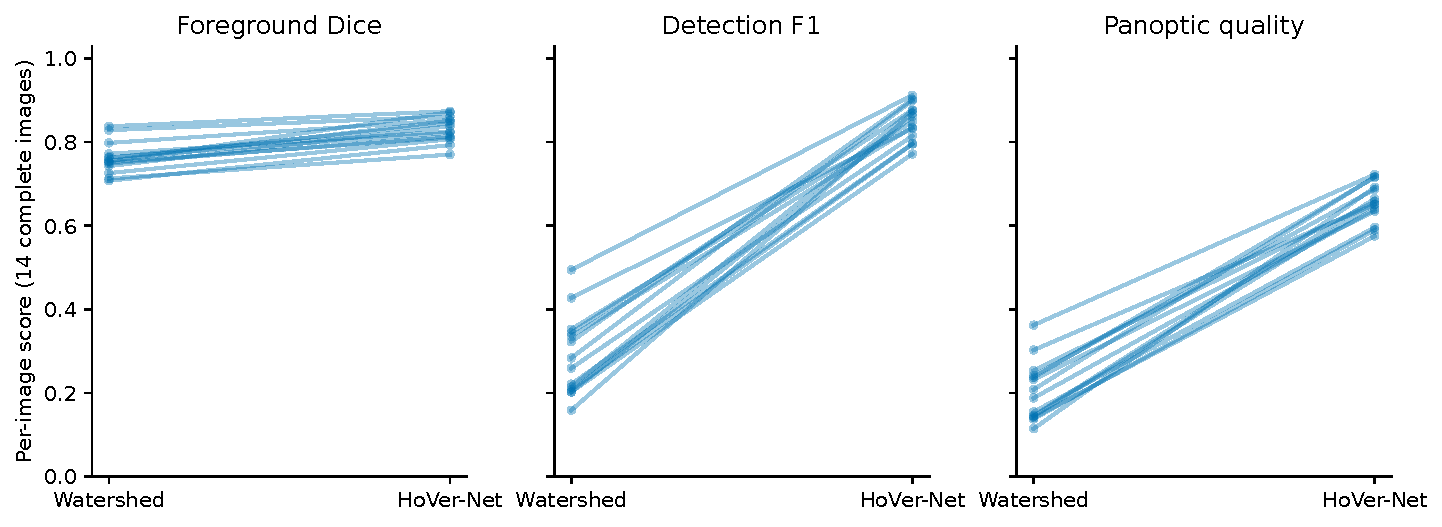
\includegraphics[width=\linewidth]{figures/segmentation.pdf}
\caption{Paired per-image segmentation scores on all 14 MoNuSeg test images. Each line represents one image, not a confidence interval.}\label{fig:segmentation}
\end{figure}

\subsection{GNNExplainer sensitivity}
At the 10\% node budget, mean confidence drops are 3.76 versus 1.29 percentage points for GCN, 5.43 versus 1.52 for GraphSAGE, and 3.36 versus 1.07 for GATv2 (explainer versus random). Differences favor the explainer at all three budgets and for all architectures (Figure~\ref{fig:gnn}). All nine descriptive paired bootstrap intervals lie above zero. This supports local node-ranking sensitivity for the chosen feature replacement, without validating the learned edge masks or establishing tissue-specific explanation quality.
\begin{figure}[tbp]\centering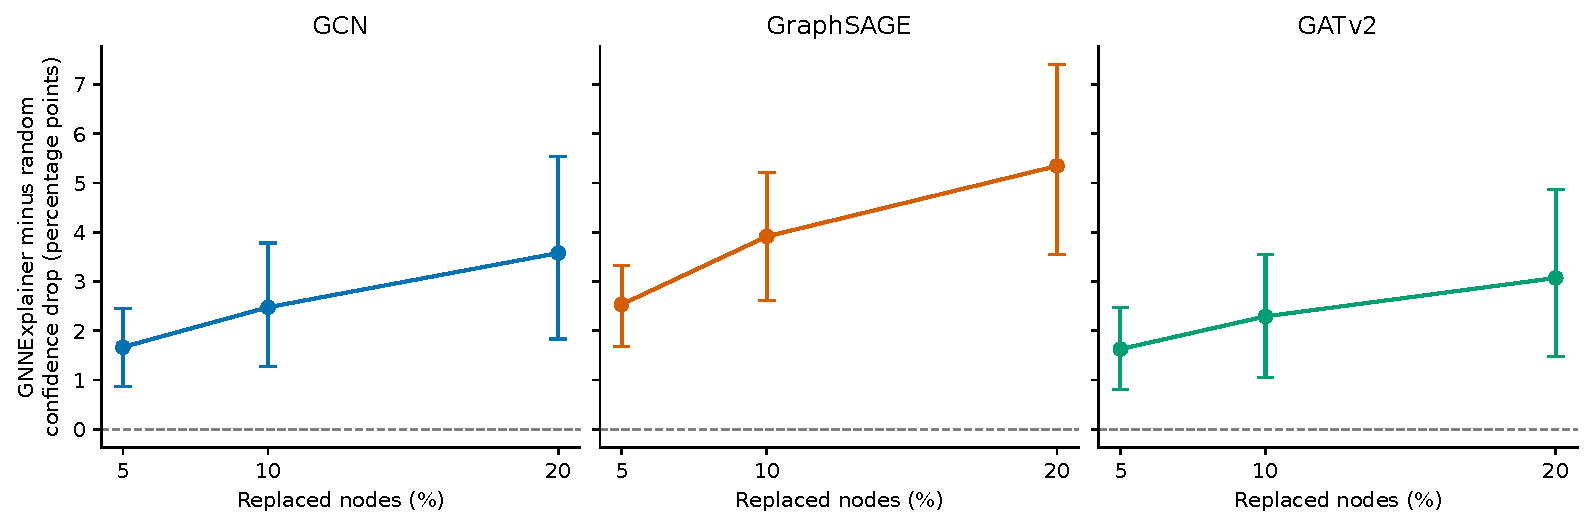
\includegraphics[width=\linewidth]{figures/gnnexplainer.pdf}
\caption{Excess predicted-class confidence drop over random node replacement. Error bars are descriptive patient-bootstrap 95\% intervals after averaging explanation seeds.}\label{fig:gnn}
\end{figure}

\subsection{Morphology encoding and numerical influence}
Mean nuclear area is strongly decodable ($R^2=0.988$, 0.980 and 0.983 for GCN, GraphSAGE and GATv2), while eccentricity and solidity are also decodable (Figure~\ref{fig:probes}). This result alone addresses encoding, not use.

For a 5\% increase in area with coupled axes, mean absolute IC-probability changes are 1.812, 2.139 and 1.502 percentage points, compared with 0.802, 0.884 and 0.693 points for coherent controls. Excess effects are respectively 1.011 [0.765, 1.255], 1.255 [0.994, 1.494] and 0.809 [0.625, 0.979] points. The decrease direction yields the same qualitative ordering (Figure~\ref{fig:gcia}). Target probe changes follow the intended direction for all evaluated patients in both directions. Collateral probe changes are recorded rather than assumed absent.

These observations support sensitivity to the coupled nuclear-size features beyond the chosen controls. Feature-range membership and successful probe movement are insufficient to establish valid intervention geometry, selective concept manipulation, or biological causality.
\begin{figure}[tbp]\centering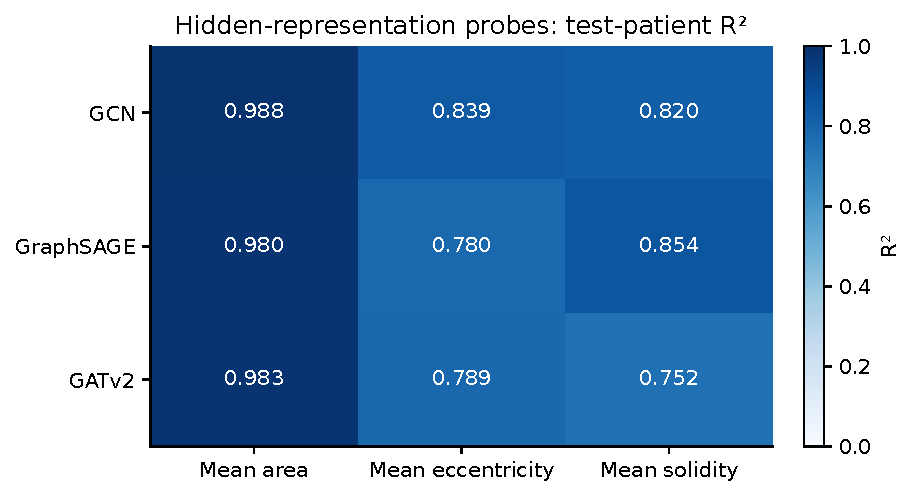
\includegraphics[width=.8\linewidth]{figures/probes.pdf}
\caption{Test-patient decoding of segmentation-derived morphology from the frozen hidden graph representations. High decoding scores are not intervention effects.}\label{fig:probes}
\end{figure}
\begin{figure}[tbp]\centering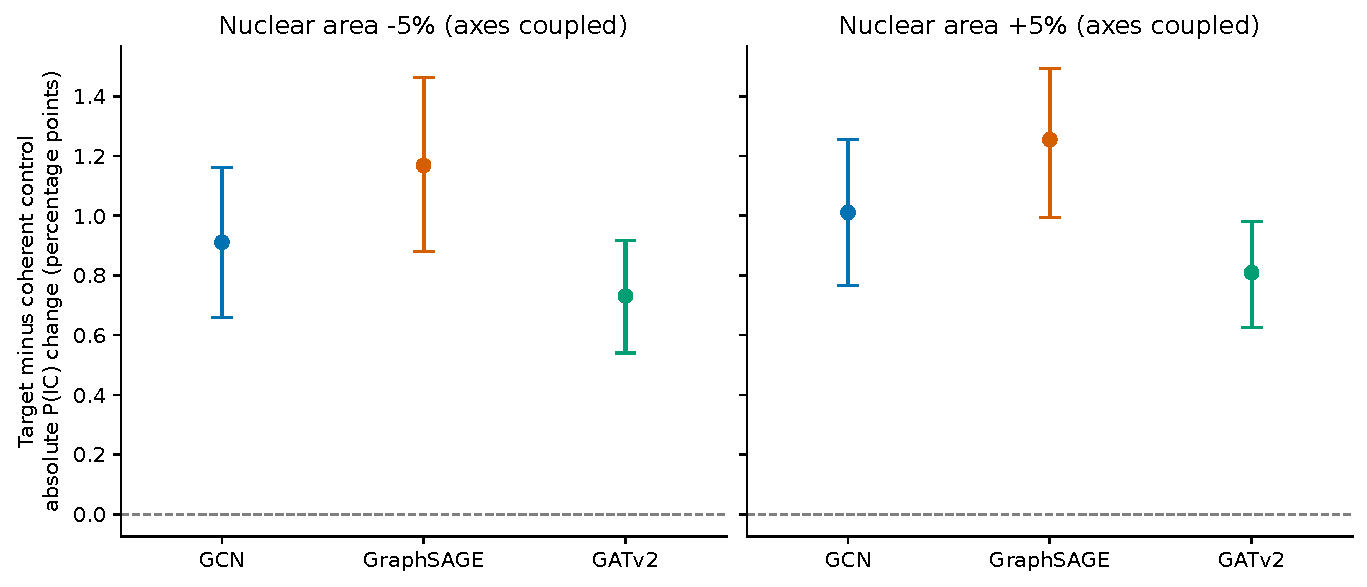
\includegraphics[width=\linewidth]{figures/gcia_controls.pdf}
\caption{Excess absolute IC-probability change over coherent, per-node norm-matched random controls. Both area directions are shown. This is supplementary numerical sensitivity analysis, not clinically validated concept faithfulness.}\label{fig:gcia}
\end{figure}

\section{Discussion}
The pilot supports a restricted GCIA premise: a concept audit can quantify both recoverability from a representation and sensitivity to an associated intervention. We observe strong morphology decoding and larger prediction changes under coupled size interventions than under random controls. However, the experiment does not identify a validated category of ``encoded but unused'' pathological concepts, nor does it isolate area from axis lengths. It therefore does not confirm the full hypothesis of selective reliance on pathologist-grounded concepts.

The change from independent to coherent random controls materially increases control effects, illustrating why perturbation structure must be matched as well as norm. The remaining excess may reflect sensitivity to a correlated feature direction; it cannot be interpreted as a causal effect of changing nuclear size in real tissue. The apparent ease of decoding area is also unsurprising when area is an explicit node input and graph representations are mean-pooled.

Key limitations are the small, size-biased sample; normal-versus-invasive extremes rather than complete breast diagnosis; the historical test's repeated use; unverified local crop labels; missing BRACS segmentation annotations; uncertain physical scale; possible MoNuSeg--PanNuke source overlap; and the absence of expert plausibility review. The exclusion of one training crop is traceable but can introduce selection bias. External BACH validation, tissue- and spatial-concept audits, validated pixel/structure interventions on these classifiers, and model-randomization sanity checks remain future work. Confidence intervals describe only the sampled patients and should not be treated as confirmatory population evidence.

\section{Conclusion}
GCIA receives partial, exploratory support as an audit of encoded morphology and numerical model sensitivity. GNNExplainer node rankings outperform random feature replacement in this experiment, and coupled nuclear-size interventions affect predictions beyond coherent numerical controls. Clinically grounded, selective interventional faithfulness remains unproven. The appropriate output is a reproducible pilot with explicit limitations, not the original full multi-cohort clinical claim.

\section*{Reproducibility and declarations}
The accompanying archive contains vector and raster figures, data-derived tables, numerical result files and SHA256 provenance. Local experiment scripts are \texttt{audit\_cell\_xai.py}, \texttt{cell\_xai\_coherent\_controls.py}, \texttt{evaluate\_nuclei.py}, and \texttt{train\_cell\_gnns.py}. No retraining is performed during figure generation. Histology images and model weights are not redistributed in this manuscript archive. Source dataset conditions apply. Authors must complete authorship, affiliations, funding, conflicts of interest, ethics/data-use statements and repository availability before submission; no expert review or ethics approval is asserted here.

\appendix
\section{Complete intervention comparisons}
All values below are probability percentage points, except node budgets and area percentages. Intervals are descriptive paired patient-bootstrap intervals.
\begin{table}[htbp]\centering\small
\begin{tabular}{lrrrr}\toprule Model & Nodes (\%) & Explainer & Random & Difference [95\% CI] \\ \midrule
GCN & 5 & 2.33 & 0.67 & 1.67 [0.88, 2.46] \\
GCN & 10 & 3.76 & 1.29 & 2.48 [1.27, 3.78] \\
GCN & 20 & 6.02 & 2.45 & 3.58 [1.83, 5.55] \\
GraphSAGE & 5 & 3.32 & 0.79 & 2.53 [1.69, 3.33] \\
GraphSAGE & 10 & 5.43 & 1.52 & 3.91 [2.62, 5.21] \\
GraphSAGE & 20 & 8.21 & 2.87 & 5.35 [3.55, 7.41] \\
GATv2 & 5 & 2.17 & 0.54 & 1.63 [0.81, 2.48] \\
GATv2 & 10 & 3.36 & 1.07 & 2.29 [1.05, 3.56] \\
GATv2 & 20 & 5.14 & 2.07 & 3.07 [1.48, 4.87] \\
\bottomrule
\end{tabular}

\caption{All GNNExplainer budgets and architectures.}
\end{table}
\begin{table}[htbp]\centering\small
\resizebox{\linewidth}{!}{\begin{tabular}{lrrrr}\toprule Model & Area change & Target & Coherent control & Difference [95\% CI] \\ \midrule
GCN & -5\% & 1.766 & 0.854 & 0.911 [0.660, 1.162] \\
GCN & +5\% & 1.812 & 0.802 & 1.011 [0.765, 1.255] \\
GraphSAGE & -5\% & 2.091 & 0.923 & 1.168 [0.879, 1.463] \\
GraphSAGE & +5\% & 2.139 & 0.884 & 1.255 [0.994, 1.494] \\
GATv2 & -5\% & 1.469 & 0.737 & 0.731 [0.540, 0.916] \\
GATv2 & +5\% & 1.502 & 0.693 & 0.809 [0.625, 0.979] \\
\bottomrule
\end{tabular}
}
\caption{Both size-intervention directions against coherent controls. Independent-control results and signed changes remain in the numerical archive.}
\end{table}

\begin{thebibliography}{9}
\bibitem{ying2019} R. Ying, D. Bourgeois, J. You, M. Zitnik and J. Leskovec. GNNExplainer: Generating Explanations for Graph Neural Networks. NeurIPS, 2019. \url{https://arxiv.org/abs/1903.03894}.
\bibitem{magister2021} L. C. Magister, D. Kazhdan, V. Singh and P. Li\`o. GCExplainer: Human-in-the-Loop Concept-based Explanations for Graph Neural Networks. 2021. \url{https://arxiv.org/abs/2107.11889}.
\bibitem{brancati2022} N. Brancati et al. BRACS: A Dataset for BReAst Carcinoma Subtyping in H\&E Histology Images. Database, 2022, baac093. \url{https://doi.org/10.1093/database/baac093}.
\bibitem{graham2019} S. Graham et al. HoVer-Net: Simultaneous Segmentation and Classification of Nuclei in Multi-Tissue Histology Images. Medical Image Analysis, 58:101563, 2019. \url{https://arxiv.org/abs/1812.06499}.
\bibitem{monuseg} N. Kumar et al. A Multi-organ Nucleus Segmentation Challenge. IEEE Transactions on Medical Imaging, 2019. Official data portal: \url{https://monuseg.grand-challenge.org/Data/}.
\end{thebibliography}
\end{document}
